\documentclass[../../main.tex]{subfiles}

% 

\begin{document}
\chapter{Spektroskopia žiarenia gama}

\section{Okienko do histórie}
Žiarenie gama je elektromagnetické žiarenie vznikajúce pri rádioaktívnych rozpadoch atómových jadier. Tvoria ho fotóny s energiou okolo $1\:\unit{MeV}$ a vyššou. Rozpad atómových jadier, pri ktorých vzniká gama žiarenie sa nazýva gama rozpad. Rozdiel medzi $\gamma$ žiarením a r\"{o}ntgenovým žiarením je hlavne v energii, ktorú fotóny nesú, no tiež v tom, že zatiaľ čo r\"{o}ntgenové žiarenie je emitované pri prechodoch elektrónov v atómovom obale, $\gamma$ je emitované pri prechodoch nukleónov v jadre.

Gama žiarenie bolo objavené francúzskym chemikom a fyzikom Paulom Villardom v roku 1900. Villard študoval žiarenie emitované rádiom Ra. Všimol si, že ním opísané žiarenie bolo silnejšie, ako už známe žiarenia (napr. beta a alfa). Villard ale nepredpokladal, že sa jedná o iný druh žiarenia. Na to prišie až Ernest Rutherford v roku 1903, ktorý následne pomenoval toto žiarenie \textit{gama} v analógii s predchádzajúcimi dvomi typmi žiarenia. Tieto žiarenia tak boli nazvané podľa ich prenikavosti látkou, teda alfa ako najmenej prenikavé, ďalej beta a gama ako najprenikavejšie žiarenie. Rutherford si tiež všimol, že gama žiarenie nie je ovplyvniteľné magnetickým poľom, čo ho potvrdilo v tom, že sa jedná o úplne nový typ žiarenia.

\section{Interakcie gama žiarenia s hmotou}

Interakciu gama žiarenia s hmotou môžeme rozdeliť nasledovne:
\begin{enumerate}
\item Primárna interakcia
\begin{enumerate}
\item koherentný rozptyl (Rayleighov rozptyl)
\item nekoherentný rozptyl (Comptonov rozptyl)
\item fotoelektrický jav
\item produkcia páru elektrón-pozitrón
\item celkové pohltenie gama žiarenia v látke
\end{enumerate}
\item Sekundárna interkacia
\begin{enumerate}
\item R\"{o}ntgenové žiarenie
\item Augerove elektróny
\item anihilácia pozitrónu a elektrónu
\item brzdné žiarenie
\end{enumerate}
\end{enumerate}

Z týchto typov interakcií sú pre meranie žiarenia dôležité iba \textit{fotoefekt}, \textit{Comptonov rozptyl} a \textit{produkcia páru}. Všetky tri procesy vedú ku kompletnému alebo čiastočnému prenosu energie fotónu na energiu elektrónu. To znamená, že dopadajúci fotón je buď pohltený, alebo je rozptýlený pod určitým uhlom. 

\subsection{Fotoelektrický jav}

Fotoefekt (alebo tiež fotoelektrický jav) je proces, pri ktorom fotón interaguje s elektrónom v atómovom obale, fotón je kompletne pohltený a elektrón získa dostatočnú energiu na uniknutie z atómového obalu. Táto interakcia ale prebieha s atómom ako celkom a preto nemôže nastať fotoefekt na voľnom elektróne. Fotoefekt fotónov s dostatočnou energiou prebieha s najväčšou pravdepodobnosťou na elektrónoch s najväčšou väzbou k jadru, teda na \textit{K} vrstve. Uvoľnený elektrón získa energiu
\begin{equation}
E_e=h\nu -E_v,
\end{equation}
kde $E_v$ je väzbová energia elektrónu a $\nu$ je frekvencia fotónu.

Fotoefekt bol po prvýkrát pozorovaný Heinrichom Hertzom v roku 1887, ktorý zistil, že elektródy osvetlené UV svetlom ľahšie iskria. V roku 1900 Max Planck navrhol hypotézu, že elektromagnetická energia je prenášaná po kvantách. V roku 1905 Albert Einstein publikoval článok s hypotézou, že svetelná energia je prenášaná v diskrétnych kvantách a objasnil tým experimentálne výsledky. V roku 1914 Robert Milikan experimentálne potvrdil Einsteinovu hypotézu a obaja boli ocenený Nobelovou cenou\footnote{Einstein v roku 1921 a Milikan v roku 1923}.

Fotoelektrický jav zanechá atóm s prázdnym miestom na jednej z jeho vrstiev. Táto medzera je rýchlo zaplnená voľným elektrónom z média a následným preusporiadaním elektrónov vo vrstvách. Pri tomto záchyte tak môže dôjsť k vyžiareniu jedného alebo viacerých r\"{o}ntgenových fotónov. Toto r\"{o}ntgenové žiarenie môže opäť vyvolať fotoefekt na slabšie viazaných elektrónoch (na vonkajších vrstvách). V časti prípadov je však miesto r\"{o}ntgenového žiarenia vyžiarený Augerov elektrón.

\subsubsection{Príklad:} Uvažujme fotóny s energiou $\sim 30\:\unit{keV}$, ktoré vytvárajú fotoefekt na xenóne. 
\begin{itemize}
\item $86\%$ fotónov interaguje na K vrstve
\begin{itemize}
\item $87,5\%$ vytvára r\"{o}ntgenové žiarenie
\item $12,5\%$ vytvára Augerove elektróny
\end{itemize}
\item $14\%$ fotónov interaguje na ďalších vrstvách, pričom vznikajúce r\"{o}ntgenové žiarenie a Augerove elektróny majú nižšiu energiu
\end{itemize}

Fotoelektrický jav je dominantný proces pre gama žiarenie s (relatívne) nízkou energiou. Pravdepodobnosť procesu je zvýšená pre absorpčné materiály s veľkým atómovým číslom $Z$. Neexistuje presný analytický výraz na vyjadrenie tejto pravdepodobnosti, no veľmi dobrá je aproximácia
\begin{equation}
\tau \cong const \cdot \dfrac{Z^n}{E_\gamma^{3,5}},
\end{equation}
kde $n$ je číslo medzi $4-5$ ktoré sa lýši v závislosti od toho, akú oblasť energií skúmame a tiež na akej vrstve sa fotoelektrón nachádza.  

\begin{figure}[h!]
\centering
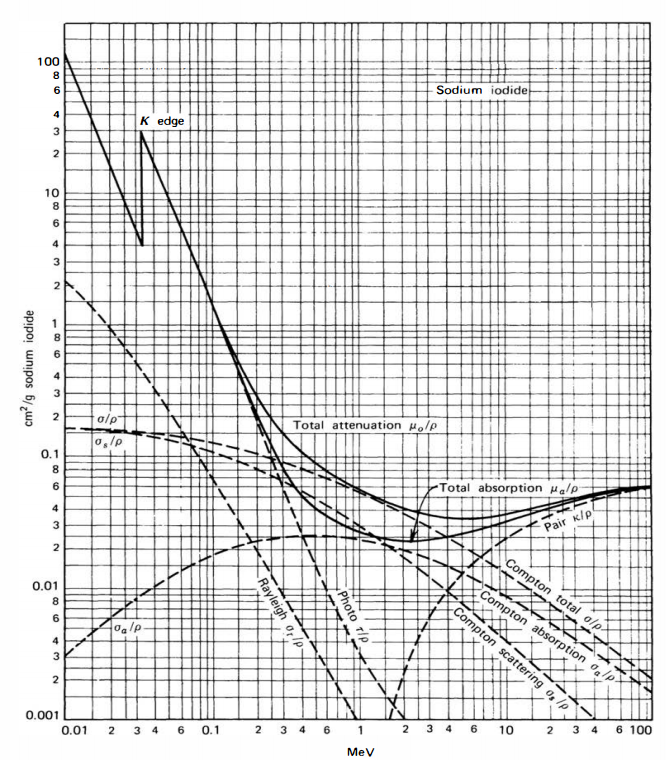
\includegraphics[width=0.75\textwidth]{js1-gama-crossections.png}
\caption{Závislosť niektorých procesov gama žiarenia na energii v NaI.}
\label{js1:img:interakcie}
\end{figure}

\subsection{Comptonov rozptyl}

Comptonov (nekoherentný) rozptyl je rozptyl medzi gama žiarením a elektrónom v materiály. Tento proces je dominantný pre oblasť energií typických pre rádioizotopické zdroje.

Pri tomto procese je nalietavajúci gama fotón odklonený o uhol $\theta$ oproti pôvodnému smeru. Časť energie fotónu sa prenesie na elektrón (ktorý bol na počiatku v kľude), ktorý nazývame \textit{recoil} elektrón. Ten sa dostane do pohybu pod uhlom $\phi$ oproti pôvodnému smeru fotónu. Vzhľadom na to, že sú povolené všetky môžné veľkosti uhla $\theta$, energia, ktorú fotón predá elektrónu, môže nadobúdať hodnoty od $0$ až po veľkú časť energie fotónu.

Comptonov rozptyl objavil Arthur Holly Compton v roku 1923\footnote{za čo bol v roku 1927 odmenený Nobelovou cenou}. Vo svojom pôvodnom experimente (viď obr. \ref{js1:img:experiment}) nechal ožarovať grafitový terčík r\"{o}ntgenovým žiarením. Po rozptýlení nasledovala štrbina, ktorá určovala presný uhol, pod ktorým sa fotón rozptýlil. Energiu rozptýleného fotónu nakoniec určoval pomocou Braggovho rozptylu na kryštály. Na konci bola ionizačná komora, kde však mohol merať iba celkovú energiu, nie energiu jednotlivého fotónu. Rozdiel vlnových dĺžok fotónov pred a po rozptyle nazývame Compotonov posun.

\begin{figure}[h!]
\centering
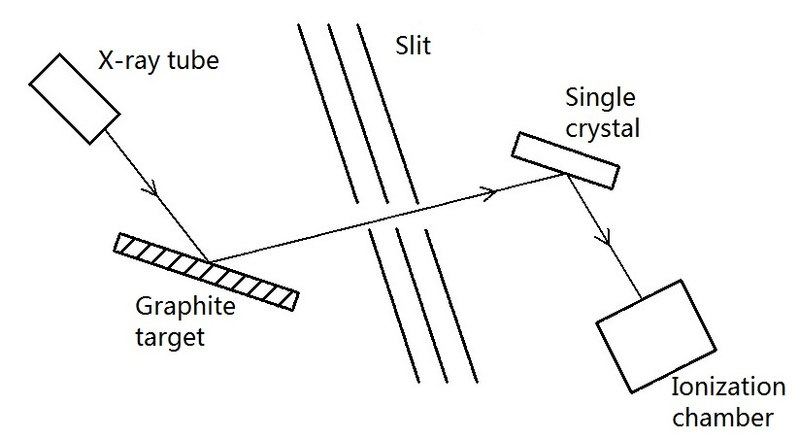
\includegraphics[width=0.5\textwidth]{js1-comptonexperiment.jpg}
\caption{Schéma pôvodného Comptonovho experimentu.}
\label{js1:img:experiment}
\end{figure}

\begin{figure}[h!]
\centering
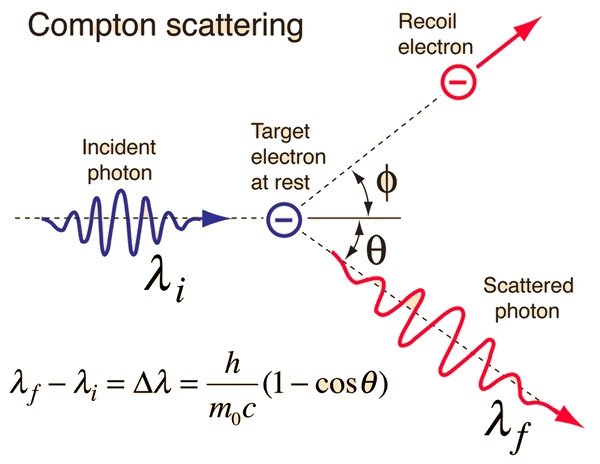
\includegraphics[width=0.5\textwidth]{js1-compton.png}
\caption{Schéma Comptonovho rozptylu.}
\end{figure}

Energiu fotónu po rozptýlení možno veľmi jednoducho odvodiť zo zákonov zachovania hybnosti a energie. Uvažujme relativistický rozptyl:
\begin{subequations}
\begin{equation}
h\nu+m_ec^2=h\nu'+\sqrt{(m_ec^2)^2+(pc)^2}
\end{equation}
\label{js1:eq:compton}
\begin{equation}
\dfrac{h\nu}{c}=\dfrac{h\nu'}{c}\cos\theta+p\cos\phi
\end{equation}
\begin{equation}
0=\dfrac{h\nu'}{c}\sin\theta-p\sin\phi
\end{equation}
\end{subequations}
Druhú a tretiu rovnicu\footnote{jedná sa o zákon zachovania hybnosti v smere $x$ a $y$} prenásobíme $c$, prehodíme členy s $\nu'$ na druhú stranu a umocníme, následne sčítame:
\begin{subequations}
\begin{equation*}
(h\nu)^2-2h^2\nu\nu'\cos\theta+(h\nu')^2\cos^2\theta=p^2c^2\cos^2\phi
\end{equation*}
\begin{equation*}
(h\nu')^2\sin^2\theta=p^2c^2\sin^2\phi
\end{equation*}
\end{subequations}

\begin{equation*}
(h\nu)^2+(h\nu')^2-2h^2\nu\nu'\cos\theta=(pc)^2
\end{equation*}

Teraz za $pc$ dosadíme do rovnice (\ref{js1:eq:compton}) a umocníme rovnicu:
\begin{equation*}
(h\nu)^2+(m_ec^2)^2+(h\nu')^2+2h\nu m_ec^2-2h^2\nu\nu'-2h\nu' m_ec^2=(m_ec^2)^2+(h\nu)^2+(h\nu')^2-2h^2\nu\nu'\cos\theta
\end{equation*}
\begin{equation*}
h\nu m_ec^2-h^2\nu\nu'-h\nu' m_ec^2=-h^2\nu\nu'\cos\theta
\end{equation*}
\begin{equation*}
h\nu'\left( h\nu(1-\cos\theta)+m_ec^2\right)=h\nu m_ec^2
\end{equation*}

Výsledná formula má tvar
\begin{equation}
h\nu '=\dfrac{h\nu}{1+\dfrac{h\nu}{m_ec^2}(1-\cos\theta)},
\end{equation}
kde $m_ec^2=511\:\unit{keV}$ je pokojová energia elektrónu. Zo vzťahu vyplýva, že pre malé uhly $\theta$ je zmena energie fotónu malá. 

\begin{figure}[h!]
\centering
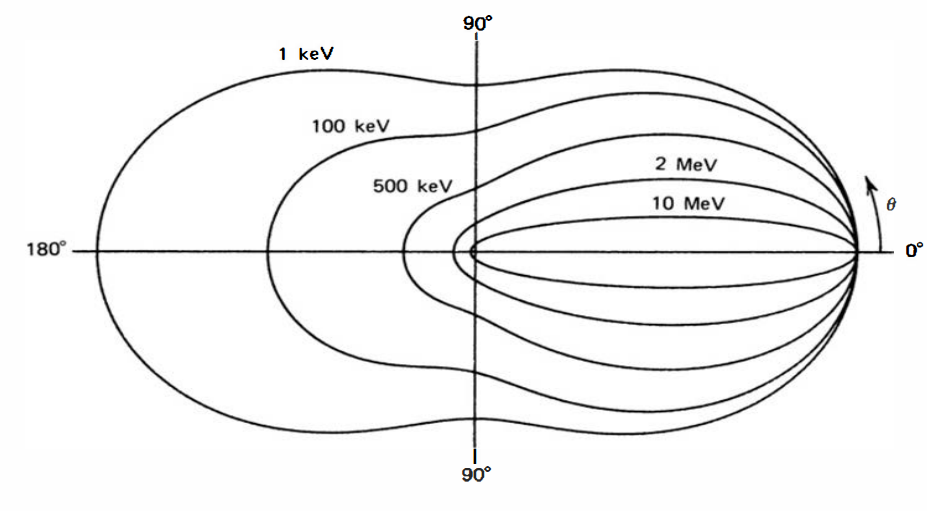
\includegraphics[width=0.7\textwidth]{js1-compton-rozneenergie.png}
\caption{Azimutálne rozdelenie rozptýlených fotónov od energie nalietavajúceho fotónu}
\label{js1:img:compton-rozneenergie}
\end{figure}



Pravdepodobnosť Comptonovho rozptylu závisí od počtu elektrónov v atómovom obale, teda rastie lineárne so $Z$. Energetická závislosť Comptonovho rozptylu je tiež znázornená na obr. \ref{js1:img:interakcie}. Celkový diferenciálny účinný prierez Comptonovho rozptylu môžeme vyjadriť pomocou \textit{Klein-Nishinaovej formuly}
\begin{equation}
\dfrac{\mathrm{d\sigma}}{\mathrm{d}\Omega}=Zr_e^2\left( \dfrac{1}{1+\alpha(1-\cos\theta)}\right)^2\left(\dfrac{1+\cos^2\theta}{2}\right)\left(1+\dfrac{\alpha^2(1-\cos\theta)^2}{(1+\cos^2\theta)\left[ 1+\alpha(1-\cos\theta)\right] }\right),
\end{equation}
kde $\alpha=h\nu /(m_ec^2)$ a $r_e$ je polomer elektrónu. Toto rozdelenie je znázornené na obr. \ref{js1:img:compton-rozneenergie}.


\subsection{Produkcia páru}

Pokiaľ má fotón dostatočnú energiu, môže sa samovoľne rozpadnúť na elektrón a pozitrón. V prípade, že sa fotón nachádza v elektromagnetickom poli atómu, prahová energia pre tento proces je $E=2m_ec^2=1,02\:\unit{MeV}$. V prípade elektromagnetického poľa elektrónu je táto energia $E=4m_ec^2=2,04\:\unit{MeV}$. Pokiaľ má fotón energiu iba o málo väčšiu, ako je prahová energia, tak je pravdepodobnosť tvorby páru malá. Tento efekt je preto dominantný pre vysoké energie (niekoľko MeV). Pri tomto procese sa fotón premení na elektrón a pozitrón a energia nad $1,02\:\unit{MeV}$ je transformovaná na kinetickú energiu tohto páru. Keďže pozitrón v médiu rýchlo anihiluje, sekundárnym produktom tohto procesu sú dva fotóny.

Neexistuje výraz, ktorý by opisoval pravdepodobnosť produkcie páru na jadro, ale amplitúda nadobúda hodnoty približne ako $Z^2$. Približné výrazy pre účinný prierez v špeciálnych prípadoch sú:
\begin{itemize}
\item pre $2m_ec^2\ll E_\gamma \ll \frac{m_ec^2Z^{1/3}}{\alpha}$
\begin{equation}
\sigma(E)=4\alpha Z^2r_e^2\left[\dfrac{7}{9}\ln\dfrac{2E_\gamma}{m_ec^2}-\dfrac{109}{54}\right]
\end{equation}
\item pre $E_\gamma \gg \frac{m_ec^2Z^{1/3}}{\alpha}$
\begin{equation}
\sigma(E)=4\alpha Z^2r_e^2\left[\dfrac{7}{9}\ln183Z^{-1/3}-\dfrac{1}{54}\right]
\end{equation}
\end{itemize}
V prípade, že fotón má veľmi veľkú energiu ($E_\gamma \gg m_ec^2$), vzniknutý pár letí dopredu, pričom ich vzájomný uhol je približne $\Theta\approx  \frac{m_ec^2}{E_\gamma}$.

\subsection{Koherentný rozptyl}
Ďalším typom rozptylu, ktorý môže nastať je koherentný rozptyl (nazývaný aj Rayleigho rozptyl). Jedná sa o proces, pri ktorom fotón reaguje s elektrónmi viazanými v atóme. Nedochádza však k excitácií ani ionizácií atómu a gama fotón pri tomto procese nestráca žiadnu energiu, preto sa často tento proces neuvažuje ako interakcia gama žiarenia. Fotón ale zmení smer hybnosti. 

Účinný prierez tejto interakcie je daný vzťahom
\begin{equation}
\sigma_R=\dfrac{8\pi}{3}r_e^2\dfrac{\nu^4}{(\nu_0^2-\nu^2)^2+(\gamma_0\nu)^2},
\end{equation}
kde výraz $\frac{8\pi}{3}r_e^2$ označujeme ako $\sigma_T$, $\nu$ je frekvencia fotónu a $\nu_0$ je rezonančná frekvencia. Môžeme si všimnúť zjednodušenie tohto výrazu v troch limitách:
\begin{subequations}
\begin{equation}
\nu \ll \nu_0 \Rightarrow \sigma_R=\sigma_T\dfrac{\nu^4}{\nu_0^4}
\label{js1:eq:modraobloha}
\end{equation}
\begin{equation}
\nu \approx \nu_0 \Rightarrow \sigma_R=\sigma_T\dfrac{\nu_0^2}{\gamma_0^2}
\end{equation}
\begin{equation}
\nu \gg \nu_0 \Rightarrow \sigma_R=\sigma_T
\end{equation}
\end{subequations}

Výraz (\ref{js1:eq:modraobloha}) nám navyše hovorí, že svetlo s nízkou energiou sa rozptyluje nepriamo úmerne štvrtej mocnine vlnovej dĺžky. To znamená, že najviac sa rozptyluje svetlo s menšími vlnovými dĺžkami, čo je v prípade viditeľného svetla modrá farba. To je dôvodom, prečo je obloha modrá.

Okrem Rayleigho rozptylu poznáme ešte Thomsonov rozptyl, ktorý opisuje koherentný rozptyl fotónu na voľnom elektróne.

\section{Detektory gama žiarenia}

\subsection{Porovnávacie charakteristiky detektorov}

V dnešnej dobe existuje veľké množstvo rôznych typov detektorov, pričom každé z nich majú rôzne vlastnosti. Keď chceme detektory medzi sebou porovnávať najčastejšie sledujeme tieto porovnávacie charakteristiky:
\begin{itemize}
\item citlivosť - schopnosť produkovať merateľný signál pre daný typ častíc a energií. Citlivosť môže závisieť od účinného prierezu reakcií, konštrukcie detektoru, šumu detektoru či hrúbke a druhu materiálu obklopujúceho citlivý objem.
\item odozva - vzťah medzi energiou častice a výstupom na detektore
\item tvar pulzu - tvar signálu z detektoru (nábežná hrana, zostupná rýchla zložka, pomalá zložka)
\item mŕtva doba - doba potrebná na vytvorenie a spracovanie signálu v detektore. Existujú dva typy mŕtvej doby. Buď sa detektor počas mŕtvej doby stane necitlivým, alebo zostáva citlivým a amplitúdy sa sčítavajú.
\item detekčná účinnosť - pomer medzi počtom častíc detekovaných detektorom a vyžiarených zdrojom. Tento pomer nazývame absolútna účinnosť, ktorá sa skladá z vnútornej a geometrickej účinnosti $\eta_{total}=\eta_{in}\eta_{geometry}$. Vnútorná účinnosť je pomer počtu častíc, ktoré boli detekované a ktoré dopadli na detektor. Geometrická účinnosť je pomer častíc, ktoré dopadli na detektor a ktoré boli vyžiarené.
\item energetické rozlíšenie - najmenší rozlíšiteľný rozdiel energie $\Delta E$ medzi dvomi blízkymi energiami.
\item pomer medzi píkom a comptonovským pozadím - pomer medzi maximálnou amplitúdou v píku $1332\:\unit{keV}$ a strednou hodnotou v oblasti $1040-1096\:\unit{keV}$.
\item FWHM - pološírka (Full Width in Half Max) úzko súvisí s energetickým rozlíšením. Pre Gaussovu krivku totiž platí $\mathrm{FWHM}=2,35\sigma$. Pološírku ovplyvňujú napr. pohltenie nosičov náboja, vlastnosti elektroniky, ...
\item časové rozlíšenie - najmenší rozlíšiteľný rozdiel časov
\item dráhové rozlíšenie - najmenší rozlíšiteľný rozdiel dráh
\item odolnosť voči radiačnému poškodeniu - menej citlivé na radiačné ožiarenie sú kvapalné a plynové detektory, viac citlivé sú scintilačné a polovodičové detektory. 
\end{itemize}

\subsection{Scintilačné detektory}

Scintilačné detektory prevádzajú absorbovanú energiu ionizujúceho žiarenia na energiu fotónov s frekvenciou v oblasti viditeľného alebo ultrafialového svetla. Historicky ide o najstarší spôsob detekcie jednotlivých ťažkých nabitých častíc, kedy záblesky tienidla pokrytého vrstvou ZnS boli počítané pomocou jednoduchého mikroskopu okom pozorovateľa. Toto zariadenie sa nazývalo spintariskop a kládlo na zrak pozorovateľa značné nároky. V roku 1909 uskutočnili Geiger a Marsden pomocou spintariskopu experiment zaoberajúci sa rozptylom $\alpha$ častíc na tenkej fólii, ktorý viedol k Rutherfordovmu objavu jadra (1911). Ďalšie informácie o histórií scintilačných detektorov nájdete v sekcii 2.4 Detektory záření.

Scintilačné detektory patria medzi najpoužívanejšie detektory ionizujúceho žiarenia. Ich výhoda spočíva okrem dobrých spektrometrických vlastností tiež v tom, že detekčné médium, scintilátor, môže mať značné rozmery a takmer ľubovoľný tvar. Základné usporiadanie scintilačného dtekčného systému je znázornené na obr. \ref{js1:img:schemascint}. 

\begin{figure}[h]
\centering
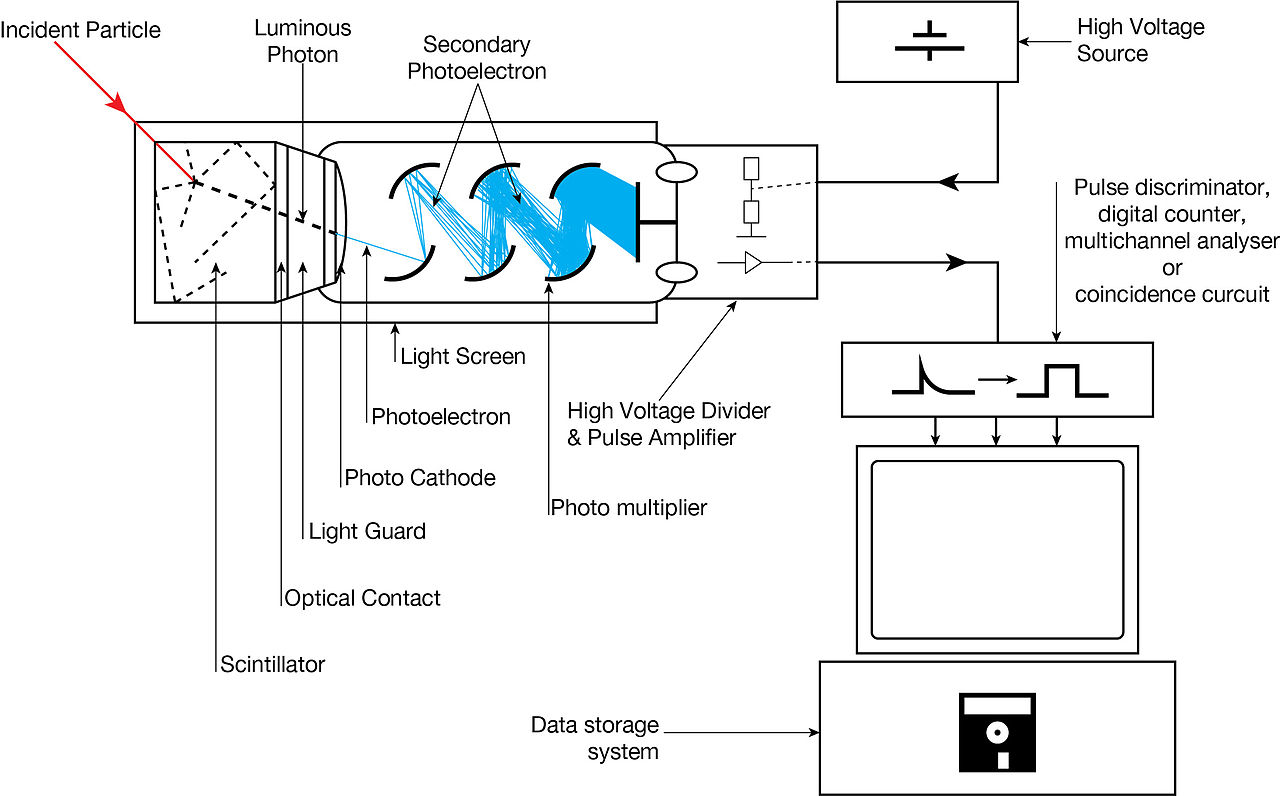
\includegraphics[width=0.7\textwidth]{js1-scint.jpg}
\caption{Schéma scintilačného detektoru.}
\label{js1:img:schemascint}
\end{figure}

Vlastné čidlo detektoru predstavuje scintilátor, v ktorom dopadajúce žiarenie spôsobuje ionizáciu a excitáciu jeho atómov a molekúl. Ich návrat do základného stavu je doprevádzaný emisiou svetelného žiarenia. Aby sa mohli svetelné fotóny maximálne využiť, obklopuje sa scintilátor \textit{reflektorom}. Zozbierané fotóny po prechode optickým kontaktom pôsobia na fotokatódu fotonásobiča. Fotóny po dopade na fotokatódu uvoľňujú fotoelektróny, ktoré sa po fokusácií a urýchlení elektrickým poľom dostávajú na prvú dynódu. Povrch dynód je pokrytý materiálom s veľkým súčiniteľom sekundárnej emisie. Vplyvom toho sa počet elektrónov opúšťajúcich každú nasledujúcu dynódu neustále zväčšuje. Výsledkom tohoto násobiaceho procesu je, že každý fotoelektrón vyvolá celkom $s$ elektrónov, ktoré sú potom zozbierané na anóde fotonásobiča. Zosílenie fotonásobiča býva v rozsahu $10^5$ až $10^9$.

Od vhodných scintilačných materiálov požadujeme nasledujúce vlastnosti: vysoká efektivita premeny kinetickej energie nabitých častíc na scintilačné fotóny, dobrá linearita konverzie - svetelný výťažok by mal byť priamo úmerný uloženej energii pre široké spektrum energií, priehľadnosť pre svoje emisné vlnové dĺžky, emisné spektrum zhodné so spektrálnou citlivosťou fotonásobiča, krátka rozpadová konštanta, dobré optické vlastnosti, dobrá opracovateľnosť, index lomu by mal byť blízky indexu lomu skla ($\sim 1,5$).

Rozdelenie scintilačných materiálov:
\begin{enumerate}
\item \textbf{Organické scintilátory} - vzhľadom k nízkej hustote a nízkemu protónovému číslu $Z$ nie sú organické scintilátory bežne používané na meranie $\gamma$ žiarenia.
\begin{enumerate}
\item organické kryštály
\begin{enumerate}
\item antracén - jedná sa o jeden z najstarších a najefektívnejších organických scintilátorov.
\end{enumerate}
\item kvapalné scintilátory - používajú sa ako $4\pi$ detektory pre meranie aktivít $\beta$ žiaričov
\item plastikové scintilátory - jedná sa o scintilačný materiál (\textit{fluor}) rozpustený v monomérnej látke (\textit{base}), ktorá môže byť následne polymerizovaná na pevný plast. Plastikové scintilátory sa veľmi ľahko vyrábajú a tvarujú, sú lacné a môžu dosahovať relatívne veľké objemy. Ako plastové zložky sa používajú najmä polystyrén (PS), polyvyniltoluén (PVT) a polymetylmetakrylát (PMMA). Ako \textit{fluory} sa bežne používajú polyfenyly a aryly oxazolu a oxadiazolu.
\end{enumerate}

\item \textbf{Anorganické scintilátory} - najčastejšie sa používajú na detekciu a spektrometriu $\gamma$ žiarenia a r\"{o}ntgenového žiarenia. 

\begin{enumerate}
\item alkalické halogenidy 
\begin{enumerate}
\item NaI(Tl) - [$38000\:\unit{\gamma/MeV}$, $230\:\unit{ns}$, $415\:\unit{nm}$]\footnote{v hranatej zátvorke je vždy uvedený svetelný výťažok, čas odozvy a vlnová dĺžka maximálnej emisie} jedná sa o najväčší objav v oblasti scintilačných materiálov. Jeho objav v roku 1948 ukázal, že tento materiál vytvára omnoho viac scintilačných fotónov ako ktorýkoľvek iný vtedy známy organický scintilátor.
\item CsI(Tl) - [$65000\:\unit{\gamma/MeV}$, $630\:\unit{ns}$, $540\:\unit{nm}$] emisné spektrum je posunuté k väčším vlnovým dĺžkam a nevyhovuje tak niektorým fotonásobičom. Výhodou oproti NaI je, že CsI nie je hygroskopický.
\end{enumerate}
\item pomalé anorganické kryštály
\begin{enumerate}
\item BGO ($Bi_4Ge_3O_{12}$) - [$8200\:\unit{\gamma/MeV}$, $300\:\unit{ns}$, $480\:\unit{nm}$] hlavnou výhodou materiálu je vysoká hustota ($7,13\:\unit{g\cdot cm^{-3}}$) a vysoké atómové číslo bizmutu (83). Jedná sa o \textit{čistý} scintilátor, teda nepotrebuje žiadny aktivátor. Je citlivejší na teplotu ako ostatné materiály $\Rightarrow$ je vynikajúci, keď je ochladený na teplotu tekutého dusíku.
\end{enumerate}
\item neaktivované rýchle anorganické kryštály
\begin{enumerate}
\item BaF$_2$ - [$9500(1400)\:\unit{\gamma/MeV}$, $630(0,6)\:\unit{ns}$, $310(220)\:\unit{nm}$]\footnote{v zátvorke sú uvedené vlastnosti rýchlej zložky} ukazuje sa, že jeho scintilačné svetlo má dve zložky - rýchla zložka s krátkou vlnovou dĺžkou a pomalá zložka s 1000-krát dlhším časom rozpadu a väčšou vlnovou dĺžkou. Pomalú zložkou možno eliminovať zvýšením teploty nad $200\unit{^\circ C}$
\item PbWO$_4$ - [$200\:\unit{\gamma/MeV}$, $6\:\unit{ns}$, $425\:\unit{nm}$] je súčasťou elektromagnetických kalorimetrov na CMS (77 000 krystálov). Výhody: veľmi rýchly čas odozvy, dobrá radiačná odolnosť, veľká hustota, nízka cena, emisné spektrum vo viditeľnej oblasti. Nevýhody: veľmi nízky sveteľný výťažok, veľká teplotná závislosť, veľký index lomu.
\end{enumerate}
\end{enumerate}

\end{enumerate}

\subsection{Polovodičové detektory}

Nevýhodou scintilačných detektorov je ich relatívne nízke energetické rozlíšenie. Jediný spôsob, ako redukovať štatistický limit energetického rozlíšenia je zvýšiť množstvo nosičov informácií prenášaných jedným pulzom. Práve polovodičové detektory dokážu generovať omnoho väčšie množstvo nosičov. Fundamentálnym nosičom informácií je elektrón-dierový pár vytvorený pozdĺž cesty, ktorou išla nabitá častica cez detektor. 

V mriežke kryštálov existujú pre elektróny energetické vrstvy. Spodná, valenčná vrstva, korešponduje s elektrónmi viazanými v atóme. Horná, vodivá vrstva, reprezentuje elektróny, ktoré sa môžu voľne pohybovať kryštálom. Práve tieto elektróny predstavujú vodivosť materiálu. Vodiče majú tieto dve vrstvy prekryté. Nevodiče majú medzi týmito vrstvami medzeru väčšiu ako $5\:\unit{eV}$. Polovodiče majú túto medzeru veľkú $\sim 1\:\unit{eV}$.

Pri ľubovoľnej nenulovej teplote je medzi elektrónmi predávaná termálna energia. Tá môže spôsobiť, že elektrón preskočí z valenčnej do vodivej vrstvy a nechá na svojom mieste dieru. Pravdepodobnosť, že sa tak stane, je daná vzťahom
\begin{equation}
P(T)=CT^{3/2}\exp\left(-\dfrac{E_g}{2kT}\right),
\end{equation}
kde $E_g$ je energetický rozdiel medzi valenčnou a vodivou vrstvou, $C$ je konštanta charakterizujúca materiál. Následne dochádza k náhodnej termálnej difúzii elektrónu aj diery preč od miesta vzniku. 

Pokiaľ umiestnime polovodič do elektrického poľa, budú elektróny aj diery priťahované po mriežke v závislosti od náboja. Ich pohyb sa bude skladať z náhodného termálneho pohybu a driftovej rýchlosti rovnobežnej s vektorom intenzity poľa. Elektróny a diery sa navyše budú pohybovať v opačných smeroch. Správanie sa pohybu diery je spôsobené tým, že do diery vždy príde elektrón, ktorý je priťahovaný elektrickým poľom a nová diera tak vznikne v smere oproti pohybu elektrónov, takže sa správajú akoby kladne nabité. Driftová rýchlosť je úmerná elektrickej intenzite, pričom ich pomer nazývame mobilita
\begin{equation}
v=\mu E
\end{equation}

Bežne sa používajú dva polovodiče: kremík a germánium. Porovnanie ich vlastností je v tabuľke \ref{js1:tab:polovodice}. V oboch je mobilita rádovo rovnaká.

\begin{table}[h]
\centering
\caption{Prehľad vlastností dvoch najpoužívanejších polovodičov.}
\begin{tabular}{|l c c|}
\hline
& Si & Ge \\ \hline
$Z$ & 14 & 32 \\
atómová hmotnosť & 28,09 & 72,60 \\
hustota $\rho\:[\unit{g/cm^3}]$ & 2,33 & 5,33 \\
energetická medzera [eV] & 1,1 & 0,7 \\
mobilita elektrónov $\mu_e\:[\unit{10^4cm^2/Vs}]$ & 2,1 & 3,6 \\
mobilita dier $\mu_d\:[\unit{10^4cm^2/Vs}]$ & 1,1 & 4,2 \\
Fano faktor $F$ & $\sim$0,09-0,12 & $\sim$0,06-0,13 \\
energia na elektrón-dierový pár [eV] & 3,76 & 2,96 \\ \hline
\end{tabular}
\label{js1:tab:polovodice}
\end{table}

Aby sme zlepšili vodivosť polovodičov, pridávajú sa do nich nečistoty. Podľa nečistoty a toho, či táto nečistota prinesie elektrón alebo dieru navyše rozdeľujeme polovodiče na typ N a typ P.

Polovodiče typu N sú také, kde je pridaný \textit{dopant}, teda atóm, ktorý má namiesto 4 valenčných elektrónov 5, čo sú prvky V. skupiny, napr. fosfor. Tieto nečistoty sú pridávané v rádoch niekoľko častíc na milión. V takom prípade dopant obsadí miesto v mriežke, kde by bol normálne kremík. Keďže je jeden elektrón navyše, tento je viazaný k atómu veľmi slabo a tak je ľahké ho uvoľniť.

Polovodiče typu P sú také, kde je pridaný \textit{akceptor}, teda atóm, ktorý má 3 valenčné elektróny (napr. bór). Tento atóm vytvorí v mriežke navyše dieru. 

Keď preletí nabitá častica polovodičom, produkuje v okolí svojej dráhy elektrón-dierové páry. Tento proces môže byť priamy, alebo nepriamy, kedy častica vyprodukuje vysokoenergetický elektrón a ten následne produkuje ďalšie elektrón-dierové páry. Relevantná vlastnosť, ktorá nás zaujíma v prípade, že chceme použiť polovodič ako detektor, je energia potrebná na tvorbu jedného elektrón-dierového páru. Táto energia sa nazýva ionizačná energia $\epsilon$ a ukazuje sa, že je nezávislá od energie žiarenia. Počet vzniknutých párov nezávisí ani na tom, či je polovodič čistý, alebo je typu P alebo N.

Hlavnou výhodou polovodičových detektorov je malá hodnota ionizačnej energie, ktorá je asi 10-krát menšia ako ionizačná energia v bežnom plynovom detektore. Vďaka tomu dokážeme vytvoriť 10-krát viac nosičov náboja, čo znamená lepšie energetické rozlíšenie. 

Okrem priemernej hodnoty sú pre nás podstatné aj fluktuácie a rozptyl počtu nosičov náboja, pretože súvisia s energetickým rozlíšením detektoru. Podobne ako v plynovom detektore, je pozorovaná štatistická fluktuácia v polovodiči menšia ako predpokladaná hodnota pre prípad, že nosiče náboja sú rozdelené podľa Poissonovho rozdelenia. Poissonov model by sedel v prípade, že by všetky vzniknuté páry pozdĺž dráhy boli nezávislé. V takom prípade by bol rozptyl rovný celkovému počtu vzniknutých párov, inak povedané $E/\epsilon$. Preto definujeme \textbf{Fano faktor} $F$, ktorý sa pridáva do Poissonovho rozdelenia, aby bol zohľadnený aj tento fakt:
\begin{equation}
F\equiv \dfrac{\text{pozorovaný štatistický rozptyl}}{E/\epsilon}
\end{equation}
Pre lepšie energetické rozlíšenie požadujeme čo najmenšiu hodnotu Fano faktoru.

Rozdiel medzi kremíkovými a germániovými detektormi je v tom, že zataľ čo kremíkové detektory nemôžu byť hrubšie ako pár milimetrov, germániové detektory môžu mať hrúbku aj niekoľko centimetrov. Vďaka tomu sa môžu využívať ako totálne absorpčné detektory pre $\gamma$ žiarenie až do niekoľkých MeV. Tieto detektory nazývame HPGe (High purity germanium). Predtým, ako boli objavené súčasné čistiace technológie, germániové kryštály neboli dostatočne čisté na to, aby sa mohli použiť na spektroskopiu. Kedysi sa preto germánium dopovalo lítiom (Ge(Li)) aby vznikla oblasť, v ktorej by mohli elektróny a diery vytvoriť merateľný signál.

\subsection{Detektorové systémy}

Rôzne detektory majú rôzne výhody a nevýhody, no ich kombináciou a rôznym usporiadaním dokážeme merať aj veci, ktoré by samotné detektory nedokázali.

\begin{enumerate}
\item Anticomptonovské spektrometre

Jedná sa o polovodičový HPGe detektor obklopený scintilačným detektorom (NaI(Tl), BGO). HPGe má vysoké energetické rozlíšenie, zatiaľ čo scintilátor má vysokú účinnosť detekcie comptonovsky rozptýlených fotónov. Takouto kombináciou sme schopní potlačiť Comptonovské pozadie až o rád. 

\begin{figure}[h]
\centering
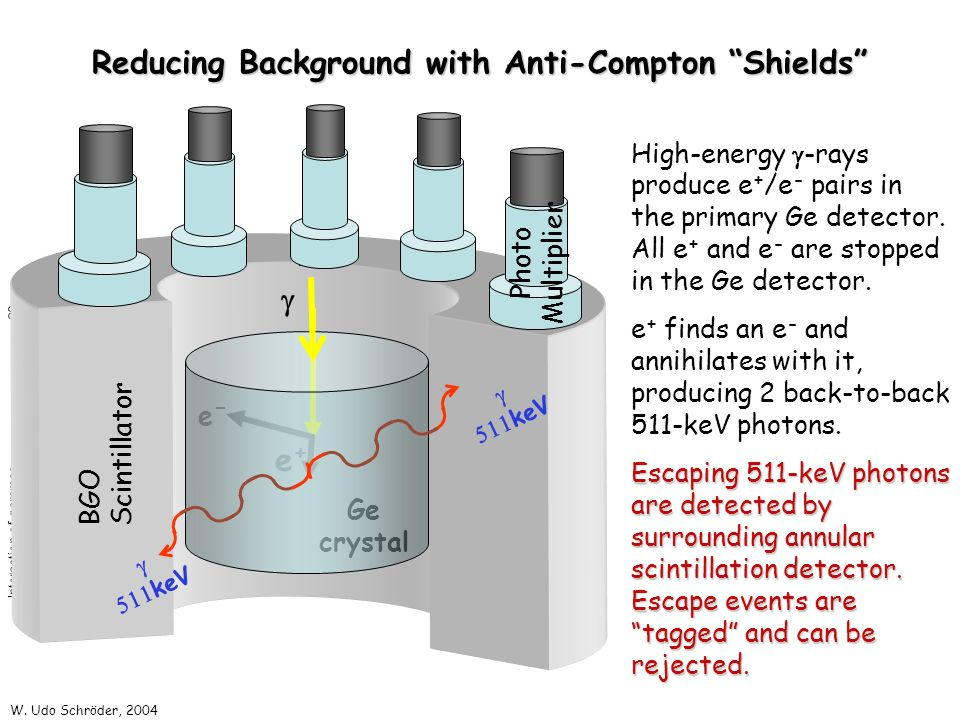
\includegraphics[width=0.7\textwidth]{js1-anticompton.jpg}
\caption{Schéma anticomptonovského spektrometra.}
\end{figure}

\item Párové spektrometre

Párový spektrometer má rovnaké usporiadanie ako anticomptonovský, teda HPGe obklopený scintilátorom. Rozdiel je v tom, že sa hľadá koincidencia HPGe a dvoch $511\:\unit{keV}$ elektrónov v scintilátore. Tým dôjde k potlačeniu všetkého okrem píku dvojného výletu. Tento postup však možno použiť iba u liniek s dostatočne vysokou energiou, aby bola dostatočne vysoká pravedpodobnosť produkcie páru. Porovnanie spektra anticomptonovského a párového spektrometra je znázornené na obr. \ref{js1:img:parovy}.

\begin{figure}[h]
\centering
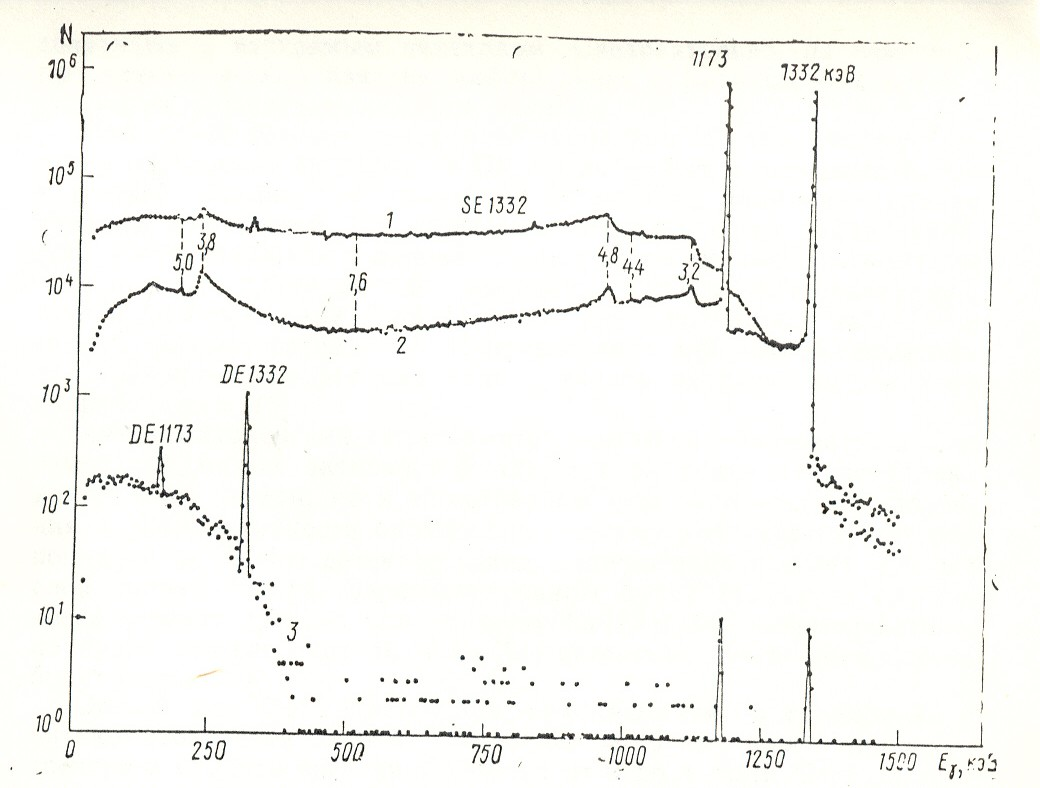
\includegraphics[width=0.6\textwidth]{js1-anticompton2.jpg}
\caption{Porovnanie jednoduchého, anticomptonovského a párového spektra určeného anticomptonovským spektrometrom. Vidíme, že pri párovom spektre dôjde k potlačeniu všetkého pri dostatočne veľkej energii.}
\label{js1:img:parovy}
\end{figure}

\item Kryštálové gule pre štúdium jadrovej štruktúry

Tieto detektorové systémy slúžia na štúdium javov s malou pravedpodobnosťou, ako napr. vysoké energie budenia jadier, vysoké momenty hybnosti, dlhé kaskády, superdeformované stavy, gigantické rezonancie, exotické jadrá, ... Prvá generácia obsahovala 6-21 HPGe detektorov s anticomptonovským tienením, BGO zostavy a kombinácie polovodičových a scintilačných detektorov. Boli to napr. TESSA3 (UK), Chateau de Cristal (FRA), OSIRIS (GER), NORDBALL (DEN). Neskôr v druhej generácií sú známe GAMMASPHERE (USA) - 70-110 HPGe detektorov s BGO tienením a $4\pi$ geometriou a európske EUROGAM a EUROBALL.

\item Scintilačné steny

Slúžia na detekciu elektromagnetických spršiek a identifikáciu vysokoenergetických fotónov. Príklady: Darmstadt (162 NaI(Tl)), DESY (672 NaI(Tl)), CLEO II (8000 CsI(Tl)), TAPS (384 BaF$_2$). Využívajú sa na detekciu fotónov od stoviek keV až po desiatky GeV. Na ALICi sa pripravuje fotónový spektrometer PHOS zostavený z kryštálov PbWO$_4$.

\begin{figure}[h]
\begin{subfigure}[b]{0.45\textwidth}
\centering
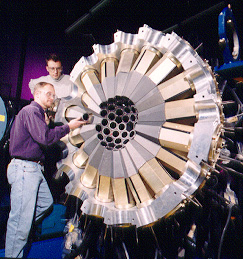
\includegraphics[width=0.8\textwidth]{js1-gamasphere.jpg}
\end{subfigure}
\begin{subfigure}[b]{0.45\textwidth}
\centering
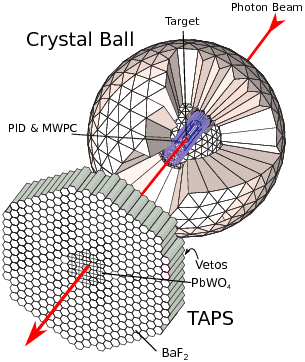
\includegraphics[width=0.7\textwidth]{js1-taps.png}
\end{subfigure}
\caption{Naľavo: kryštálová guľa GAMMASPHERE. Napravo: kombinácia kryštálovej gule a scintilačnej steny TAPS.}
\label{js1:img:gamasphere}
\end{figure}
\newpage
\item PET kamery

Pozitrónová emisná tomografia umožňuje urobiť 3D obrázky orgánov pacienta. Detektory zachytávajú koincidenciu dvojice anihilačných kvánt $511$ keV. Dve súradnice sú dané polohou dopadu fotónu, tretia súradnice sa určí z rozdielu času detekcie dvojice fotónov.
\end{enumerate}

\section{Spektrum gama žiarenia}

Spektrum gama žiarenia má niekoľko charakteristických oblastí. Aby som to vysvetlil po lopate, takto vidí monofrekvenčné fotóny polovodičový detektor. Detektor nezaznamenáva energiu fotónu, ale energiu elektrónov. Nie vždy je všetka energia fotónu predaná elektrónu a preto vidíme v spektre oveľa viac ako len fotopík.

\begin{figure}[h]
\centering
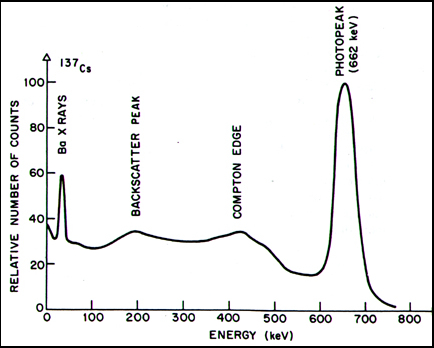
\includegraphics[width=0.7\textwidth]{js1-gamaspectrum.jpg}
\caption{Typické spektrum gama žiarenia, konkrétne pre $^{137}$Cs.}
\end{figure}

\begin{enumerate}
\item Pík úplného pohltenia (fotopík)

Pri fotoefekte je celá energia fotónu absorbovaná elektrónom pôvodne viazaným k atómu. Ten je vyrazený zo svojej pôvodnej dráhy a odnáša vo forme kinetickej energie takmer celú energiu absorbovaného fotónu. Atóm, z ktorého bol fotoelektrón vyrazený, emituje buď charakteristické žiarenie alebo Augerove elektróny. Absorpciou fotoelektrónu a vybudeného žiarenia alebo Augerových elektrónov vznikajú v rôznych miestach scintilátoru prakticky súčasne dve scintilácie, ktoré sú vyhodnotené ako jedna odpovedajúca ich súčtu a teda aj súčtu energií jednotlivých častíc. Odpovedajúce impulzy vytvárajú pík úplného pohltenia - práve tento pík je jediným nositeľom spektrometrickej informácie.

\item Comptonovské kontinuum a Comptonovská hrana

Pri Comptonovom jave interaguje fotón s voľným (slabo viazaným) elektrónom. Comptonovské elektróny sú v scintilátore zabrzdené a vyvolávajú scintilácie úmerné svojim energiám, rozptýlené fotóny ale nemusia interagovať a môžu z detektoru uniknúť. Comptonovské elektróny vytvárajú v spektru Comptonovské kontinuum, ktorá vyjadruje ich energetické rozlíšenie. Toto kontinuum je spojité a je zakončené Comptonovskou hranou. Jedná sa teda o energiu elektrónu, ktorú získa elektrón pri rozptyle. Comptonovská hrana tak značí maximálnu energiu, ktorú môže elektrón získať od fotónu (v prípade, že sa fotón rozptýli o maximálny uhol, teda $180^\circ$) a rozdiel medzi fotopíkom a Comptonovskou hranou tvorí energia fotónu, ktorý zbytok energie môže odniesť preč bez ďalšej interakcie.

\item Anihilačné píky

Fotóny s energiou $>2\cdot 511$ keV môžu vytvárať tiež pár elektrón-pozitrón. Kinetická energia páru je pri jeho zabrzdení predaná scintilátoru. Dve anihilačné kvantá môžu so scintilátorom interagovať buď priamo pomocou fotoefektu alebo jedno- či viacnásobným Comptonovským rozptylom, alebo môžu zo scintilátoru uniknúť. V prvom prípade je odozva úmerná energii primárneho fotónu a dáva tak príspevok do píku úplného pohltenia. Ak je absorbované iba jedno anihilačné kvantum a druhé unikne, vzniká v spektre \textit{prvý anihilačný pík}, ležiaci o $511$ keV nižšie ako fotopík. V prípade úniku oboch kvánt v spektre pozorujeme druhý anihilačný pík, ktorý leží o $1022$ keV nižšie ako fotopík.

\item Pík spätného rozptylu

Nízky pík uzatvárajúci Comptonovské kontinuum sa nazýva pík spätného rozptylu a odpovedá situácií, kedy detektor prijíma fotóny, ktoré neinteragovali v citlivej časti detektora, ale až za ním a rozptýlili sa pomocou Comptonovho rozptylu o uhol blízky $180^\circ$. Takýto fotón bude následne detekovaný ako nový fotón, pričom bude mať energiu odpovedajúcu rozdielu medzi Comptonovskou hranou a fotopíkom, pretože práve toto je energia, ktorú odnesie fotón pri maximálnom rozptyle.

\item 511 keV

Ďalšia možnosť je vznik 511 keV píku. Ten môže vzniknúť v prípade, že fotón prejde citlivou časťou detektora bez interakcie a za ním vytvorí pár elektrón-pozitrón. Pozitrón potom v blízkosti citlivej časti detektora anihiluje a vytvorí pár dvoch fotónov s energiou 511 keV, ktoré vyletia presne v opačných smeroch, a tak je veľká pravdepodobnosť, že jeden z nich preletí opäť cez detektor a bude zaznamenaný. 

\end{enumerate}

\section{Spektrometria vysokoenergetického gama žiarenia}

Fotóny s energiou desiatok MeV až GeV vytvárajú elektromagnetickú spŕšku. My potrebujeme určiť celkovú energiu, smer a čas príletu pôvodného fotónu. Na to je vhodné použiť anorganické scintilátory (BGO, BAF$_2$, PbWO$_4$). Pre takto energetické fotóny je fotoefekt zanedbateľný.

Dôležitým pojmom je radiačná dĺžka. Je to charakterická konštanta závislá od materiálu spojená so stratou energie vysokoenergetických elektromagnetických častíc. Jej veľkosť možno určiť pomocou približného vzťahu
\begin{equation}
X_0=\dfrac{A}{4\alpha N_A Z(Z+1)r_e^2 \log(183Z^{-1/3})},
\end{equation}
kde $A$ a $Z$ sú atómové a hmotnostné číslo, $\alpha$ je konštanta jemnej štruktúry, $N_A$ je Avogadrova konštanta a $r_e$ je klasický polomer elektrónu. Radiačná dĺžka určuje vzdialenosť, v ktorej energia elektrónu poklesne na hodnotu $1/e$. Na zachytenie fotónu s energiou $\sim 100$ MeV je treba detektor s dĺžkou $15X_0$.

Šírka elektromagnetickej spŕšky je daná Moliérovým polomerom. Podľa definície sa jedná o polomer valca obsahujúceho priemerne $90\%$ energie spŕšky. Jeho veľkosť je rádovo v centimetroch a dá sa vypočítať z radiačnej dĺžky podľa vzťahu
\begin{equation}
R_M=0,0265X_0(Z+1,2).
\end{equation}

Uvažujme teraz, že častica sa v materiály dostane do hĺbky $x=tX_0$. Počet častíc v kaskáde rastie geometricky ako $N(t)=2^t$. Kritická energia $E_c$ je definovaná ako energia, nad ktorou dominujú pri elektróne radiačné straty nad ionizačnými. Keď energia klesne pod túto hranicu, kaskády už nebudú ďalej vznikať. Celkovú energiu si tiež môžeme vyjadriť v násobkoch kritickej energie $\epsilon=E/E_c$. Maximálna hĺbka je potom $t_{max}\sim \ln \epsilon$.

Systém sa skladá zo segmentovaných detektorov z dlhých kryštálov a priemerom rovným dvojnásobku $R_M$. Energia sa následne sčítavá z hlavného aj susedných detektorov a poloha sa určuje ako stredná hodnota súradníc.

\section{Aplikácie spektroskopie gama žiarenia}

\subsection{Aktivačná analýza}

Základná myšlienka: jadrové interakcie fotónov (alebo neutrónov či nabitých častíc) vedú na rade terčových nuklidov k vzniku rádionuklidov. Meraním ich žiarenia možno určiť prítomnosť a množstvo prvku z prítomnosti a množstva príslušného rádionuklidu. V zložitých materiáloch vzniká rada rôznych vzniklých aktivácií viacerých prvkov, ktoré sa v materiály nachádzajú, preto je nutná kvalitatívna aj kvantitatívna identifikácia rádionuklidov v zmesi.

Základný vzťah pre vzniknutú aktivitu je
\begin{equation}
A=\phi \sigma \dfrac{\Theta m N_A}{A_r} \left(1-e^{-\lambda t}\right),
\end{equation}
kde $\phi$ je príkon fluencie\footnote{Fluencia častíc je definovaná ako podiel počtu častíc d$N$, ktoré dopadli v danom bode priestoru na infinitezimálnu guľu, a plochy hlavného rezu tejto gule d$A$. Príkon fluencie je časová derivácia fluencie. Zjednodušene si to možno predstaviť ako počet častíc, ktoré prechádzajú jednotkovou plochou terčíku za jednotkový čas.} bombardujúcich častíc, $\sigma$ je účinný prierez, $\Theta$ je zastúpenie terčového nuklidu v prírodnej zmesi izotopov, $m$ je hmotnosť prvku vo vzorke, $N_A$ je Avogadrova konštanta, $A_r$ je molárna hmotnosť prvku a $\lambda$ je premenová konštanta rádionuklidu.

Po dobe $t'$ po skončení ožarovania, v ktorej sa vykonáva meranie, je aktivita sledovaného nuklidu vo vzorke $A'=A\exp(-\lambda t')$. Ak zmeriame aktivitu $A'$, môžeme si vypočítať hmotnosť daného prvku vo vzorke, pretože ostatné veličiny sú dané podmienkami experimentu.

Obvykle sa využíva porovnávacie meranie - súčasne so skúmanou vzorkou sa ožiaria štandardy obsahujúce známe množstvo sledovaných prvkou. Potom platí
\begin{equation}
m_x= \dfrac{A_x}{A_s}m_s.
\end{equation}

\subsection{Materiálový výskum na zväzku iónov}

\subsubsection{PIXE} (Particle-induced X-ray emission) je technika používaná na určenie elementárneho zloženia materiálu alebo vzorky. Keď materiál vystavíme pôsobeniu iónového zväzku (najčastejšie protónom), interakcie s atómom budú generovať r\"{o}ntgenové žiarenie. PIXE je silná, citlivá a nedeštruktívna metóda na analýzu prvkov, ktorá je v dnešnej dobe bežne používaná geológmi, archeológmi a ďalšími na pomoc pri určení veku a autenticity. Jej obrovskou výhodou je možnosť vykonávať merania pri atmosférickom tlaku. Technika bola prvýkrát popísaná v roku 1970 Svenom Johanssonom.

Dnes sa už používa aj rozšírenie tejto techniky, kedy sa zväzok fokusuje do veľmi úzkeho zväzku ($\sim 1\:\unit{\mu m}$), čo zvyšuje možnosti pri mikroskopickej analýze. Táto technika má označenie microPIXE a dokáže určiť distribúciu stopových prvkov v širokom spektre. 

Z PIXE experimentu dokážeme určiť tri typy spektra:
\begin{enumerate}
\item R\"{o}ntgenová emisia 

Bombardovaním atómu iónmi s dostatočnou energiou (niekoľko MeV) spôsobí vyrazenie elektrónu zo spodnej vrstvy elektrónového obalu. Následne sa na toto miesto dostane elektrón z vyššej vrstvy, čo spôsobí vyžiarenie fotónu s energiou odpovedajúcou r\"{o}ntgenovému žiareniu. 

\item Protónový spätný rozptyl

Protóny tiež môžu interagovať s jadrami pomocou elastických zrážok. Dôjde pritom k Rutherfordovmu rozptylu protónu do uhlov blízkych $180^\circ$. Spätný odraz nám dáva informáciu o hrúbke a zložení vzorky. 

\item Prechod protónov

Prechod protónov cez vzorku nám taktiež dáva informácie o vzorke. 
\end{enumerate}

\subsubsection{PIGE} (Particle-induced gamma-ray emission) je veľmi podobná technika pri ktorej však namiesto r\"{o}ntgenového žiarenia vzniká $\gamma$ žiarenie. 

Opäť máme protónový zväzok s energiou niekoľko MeV, ktorým ožarujeme vzorku o hrúbke niekoľkých mikrónov. Rýchle protóny však tentokrát excitujú jadrá, a tie pri deexcitácií emitujú $\gamma$ žiarenie. Dôležité sú pritom reakcie (p, $\gamma$), (p, p'$\gamma$) a (p, X$\gamma$).

\begin{figure}[h]
\centering
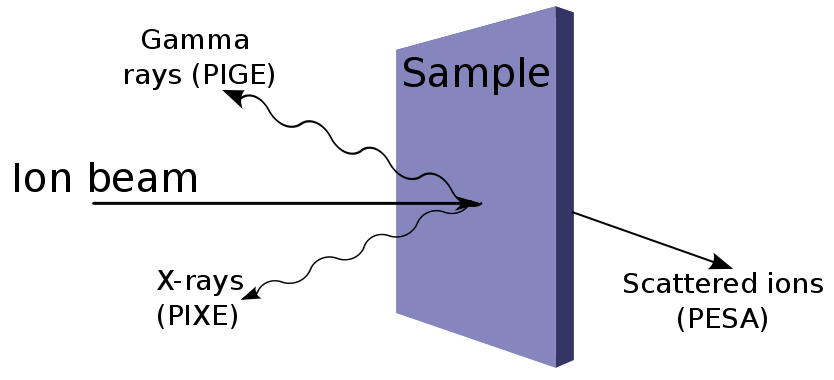
\includegraphics[width=0.7\textwidth]{js1-pixe.png}
\caption{Schéma iónového ožarovania}
\label{js1:img:pixe}
\end{figure}

Okrem PIXE a PIGE poznáme ešte PESA (Proton elastic scattering analysis), ktorá meria rozptyl ťažkých iónov (viď obr. \ref{js1:img:pixe}).

\subsection{R\"{o}ntgenová difrakčná kryštálografia}

Jedná sa o analytickú metódu zaoberajúcu sa študovaním interakcié kryštalických vzoriek s r\"{o}ntgenovým žiarením, ktorá umožňuje určiť absolútnu štruktútu molekúl, t.j. polohy atómov, dĺžky väzieb a uhly v kryštálovej mriežke.

Pri prechode monochromatického r\"{o}ntenového žiarenia látkou dochádza k difrakcii lúčov. Smer a intenzita difraktujúcich lúčov závisí na vnútornej štruktúre vzorky. V amorfnej vzorke sú atómy rozmiestnené nepravidelne a príspevky k celkovej intenzite difrakovaného žiarenia sa často vzájomne vyrušia. Naopak vzorka s periodickou štruktúrou (monokryštál) pôsobí ako difrakčná mriežka vo viditeľnom svetle. Príspevky k celkovej intenzite vzájomne interferujú a v určitých smeroch, špecifických pre konkrétnu kryštálovú štruktúru, sa sčítajú, inak sa vyrušia.

Smery a intenzity difrakovaného žiarenia sa pre vzorku zmerajä a po prevedení korekcie sa určuje absolútna štruktúra. Pri riešení sa najskôr určí hrubý model štruktúry a postupným pridávaním parametrov (anizotropia termálnych kmitov, poloha ľahkých atómov) sa optimalizuje zhoda experimentálnych dát s dátami vypočítanými podľa modelu. Miera zhody modelu s experimentálnymi dátami sa hodnotí podľa R-faktoru ale vždy je treba kritické zhodnotenie modelu človekom.

\subsection{Štúdium štruktúry jadier, jadrových premien a jadrových reakcií}

Základné metódy používané pri štúdiu štruktúry jadier sú:
\begin{enumerate}
\item určenie energií hladín a rozpadových schémat

\begin{itemize}
\item čo najpresnejšie určenie energie prechodu
\item koincidenčné meranie - určenie umiestnenia prechodu v kaskáde prechodov
\item energie hladín z reakcií
\end{itemize}

\item určenie spinov a parít hladín, multipolarity prechodov
\begin{itemize}
\item využitie výberových pravidiel pre elektromagnetické prechody - využitie výberových pravidiel a znalosti spinu niektorej z hladín, ktoré prechod spája
\item využitie pomeru medzi pravdepodobnosťou $\gamma$ prechodu a vyžiarenia konverzného elektrónu
\item využitie uhlového rozdelenia $\gamma$ žiarenia voči spinu jadra
\item uhlová korelácia dvoch fotónov vyžiarených za sebou v kaskáde
\item údaje o spine z reakcií - rôzne reakcie budia hladiny s rôznym spinom 
\end{itemize}

\item určenie pravdepodobnosti prechodu

\begin{itemize}
\item elektronické metódy - meranie krivky rozpadu
\item využitie Dopplerovho javu
\item využitie Coulombovského budenia
\end{itemize}
\end{enumerate}

Pomocou týchto metód sa skúmajú aj niektoré veľmi zaujímavé príklady

\begin{enumerate}
\item štúdium stavov s veľmi vysokým spinom

Jedná sa o stavy so spinom $I\geq 40\hbar$. Najskôr vytvoríme zložené jadro. Z neho sa vyparí niekoľko nukleónov (prevažne neutrónov) a dôjde k rýchlemu úbytku energie ($\sim 8$ MeV/n) ale malému úbytku momentu ($\sim 1\:\unit{\hbar /n}$). 

\item superdeformované stavy

Sú to stavy s vysokou deformáciou (teda s pomerom ós 2:1 a viac). Sú predpovedné vrstvovým modelom - medzery medzi vrstvami pre deformovaný potenciál.

\item gigantické rezonancie

Jedná sa o vysokofrekvenčný vzájomný korelovaný pohyb nukleónov v jadre. Pri tejto excitácií sa pohybujú vo fáze alebo v protifáze pohybujú nukleóny s rôznym spinom (spiny hore proti spinom dole) alebo izospinom (protóny proti neutrónom). 
\end{enumerate}

\end{document}